\documentclass{article}
\usepackage{amssymb, amsmath, amsthm, amscd, wasysym, graphicx, subfigure, hyperref, bm}
\usepackage{xy}
\usepackage{color}
\usepackage[procnames]{listings}

\usepackage{algorithm}
\usepackage{algpseudocode}
\usepackage{pifont}

\usepackage[skins]{tcolorbox}
\usepackage{lipsum}


\usepackage{graphicx}
%\usepackage{caption}
\usepackage{subfigure}

%%%%%%%%%%%%%%%%%%%%%%%%%%%%%
%%%%%%%%%%%%%%%%%%%%%%%%%%%%%
%%%%%%                           Title                            %%%%%%
%%%%%%%%%%%%%%%%%%%%%%%%%%%%%
%%%%%%%%%%%%%%%%%%%%%%%%%%%%%

\title{Point Estimates}
\author{}
\date{}

\addtolength{\hoffset}{-1.7cm}
\addtolength{\voffset}{-0.2cm}
\addtolength{\textwidth}{75pt}
\addtolength{\textheight}{40pt}
\addtolength{\headsep}{-5pt}
\addtolength{\topmargin}{-0pt}



\definecolor{keywords}{RGB}{200,0,200}
\definecolor{comments}{RGB}{0,0,193}
\definecolor{red}{RGB}{160,0,0}
\definecolor{green}{RGB}{0,100,0}
\definecolor{black}{RGB}{0,0,0}

\newcommand{\A}{\mathcal{A}}
\newcommand{\C}{\mathcal{C}}
\newcommand{\D}{\mathcal{D}}
\newcommand{\G}{\mathcal{G}}
\newcommand{\B}{\mathcal{B}}
\newcommand{\E}{\mathcal{E}}
\newcommand{\cS}{\mathcal{S}}
\newcommand{\U}{\mathcal{U}}
\newcommand{\cL}{\mathcal{L}}
\newcommand{\cO}{\mathcal{O}}
\newcommand{\cU}{\mathcal{U}}
\newcommand{\M}{\mathcal{M}}
\newcommand{\bN}{\mathbb{N}}
\newcommand{\bQ}{\mathbb{Q}}
\newcommand{\Exp}{\mathbb{E}}
\newcommand{\bC}{\mathbb{C}}
\newcommand{\bR}{\mathbb{R}}
\newcommand{\bZ}{\mathbb{Z}}
\newcommand{\bK}{\mathbb{K}}
\newcommand{\bF}{\mathbb{F}}

\newcommand{\fF}{\mathbf{F}}
\newcommand{\fA}{\mathbf{A}}
\newcommand{\Grp}{\mathbf{Grp}}
\newcommand{\Set}{\mathbf{Set}}
\newcommand{\Mor}{\mathrm{Mor}}
\newcommand{\Aut}{\mathrm{Aut}}
\newcommand{\Gal}{\mathrm{Gal}}
\newcommand{\Char}{\mathrm{char}}
\newcommand{\SL}{\mathrm{SL}}
\newcommand{\GL}{\mathrm{GL}}
\newcommand{\Span}{\mathrm{span}}
\newcommand{\Hom}{\mathrm{Hom}}
\newcommand{\Ext}{\mathrm{Ext}}
\newcommand{\im}{\mathrm{im}}
\newcommand{\col}{\mathrm{col}}
\newcommand{\argmax}{\mathrm{argmax}}
\newcommand{\cone}{\mathrm{cone}}
\newcommand{\rank}{\mathrm{rank}}
\newcommand{\RP}{\mathbb{R}\mathrm{P}}
\newcommand{\tr}{\mathrm{tr}}

\newcommand{\df}{\overset{\text{def}}{=}}
%\newcommand{\deg}{\mathrm{deg}}

\newcommand{\vx}{\mathbf{x}}
\newcommand{\vy}{\mathbf{y}}
\newcommand{\vu}{\mathbf{u}}
\newcommand{\vv}{\mathbf{v}}
\newcommand{\va}{\mathbf{a}}
\newcommand{\vb}{\mathbf{b}}
\newcommand{\vc}{\mathbf{c}}
\newcommand{\vd}{\mathbf{d}}
\newcommand{\vg}{\mathbf{g}}
\newcommand{\vk}{\mathbf{k}}
\newcommand{\vw}{\mathbf{w}}
\newcommand{\vz}{\mathbf{z}}
\newcommand{\vp}{\mathbf{p}}
\newcommand{\vq}{\mathbf{q}}
\newcommand{\vS}{\mathbf{S}}
\newcommand{\vf}{\mathbf{f}}
\newcommand{\bo}{\mathbf{1}}
\newcommand{\bz}{\mathbf{0}}
\newcommand{\id}{\mathrm{id}}

\theoremstyle{theorem}
\newtheorem{thm}{Theorem}

\theoremstyle{theorem}
\newtheorem{prop}{Proposition}
\theoremstyle{theorem}
\newtheorem{cor}{Corollary}

\theoremstyle{lemma}
\newtheorem{lemma}{Lemma}

\theoremstyle{definition}
\newtheorem{defn}{Definition}

\theoremstyle{example}
\newtheorem{ex}{Example}


\addtolength{\hoffset}{-1.5cm}
\addtolength{\voffset}{-1.0cm}
\addtolength{\textwidth}{90pt}
\addtolength{\textheight}{100pt}
\addtolength{\headsep}{-19pt}
\addtolength{\topmargin}{-22pt}

\begin{document}
\maketitle
\input xy
\xyoption{all}
\xyoption{arc}

\section{Data}
We work with a year of 311 service request data and, in the rest of the notebook, analyze the differences/similaritys between geographic/response time distribution between service requests generated by constituent calls and service requests generated by the Citizens Connect App.

We filter the full 311 service request data set for closed requests that are opened between $\texttt{January 01, 2015 12:00AM}$ and $\texttt{January 01, 2016 12:00AM}$. This data set is then split into $\texttt{call\_data}$, requests generated by constituent calls, and $\texttt{app\_data}$, requests generated by the Citizens Connect App. We then choose a random subset from each $\texttt{call\_data}$ and $\texttt{app\_data}$ (by randomizing and then slicing), obtaining two datasets each of approximately 20,000 data points.

For better model fitting, we standardize each feature of the pooled set of sliced $\texttt{call\_data}$ and sliced $\texttt{app\_data}$, so that each feature has mean zero and standard deviation 1. 

\section{Model Selection}
The Bayesian Information Criterion (BIC) score is a weighted difference between the log-likelihood of a model and the complexity of the model (as well as the size of the data), 
\begin{align}
\log\mathcal{L}(X | \theta^{MLE}, \mathcal{M}) - \frac{1}{2} \kappa_\mathcal{M} * \log(N),
\end{align}
where $\mathcal{L}$ is the log-likelihood of the data, $X$, given the model, $\mathcal{M}$, and the maximum likelihood parameters of the model, $\theta^{MLE}$. The BIC score approximates the evidence for the data $\log p(X | \mathcal{M})$ given the model $\mathcal{M}$, under the assumption that data distribution is an exponential family. In model selection, higher BIC scores indicate a preferable balance between fewer model parameters (preventing overfitting) and better model fit. In a Bayesian framework, we want to select the model with the largest posterior probability. This means choosing the model with the largest integrated complete likelihood (ICL). A BIC-like approximation of the ICL is proposed by Biernacki et al (\cite{Biernacki})to be 
\begin{align}
\log \mathcal{L}(X, Z | \theta^{MAP},  \mathcal{M}) -  \frac{1}{2} \kappa_\mathcal{M} * \log(N),
\end{align}
where $X$ is the data and $Z$ is the latent cluster labels.
From Figure \ref{fig:bic}, we see that the most appropriate number of clusters for MAP estimates is $K=3$.
\begin{figure}[h!]
\begin{center}
\caption{Model Selection Using BIC Scores}
\subfigure[BIC score plot for Constituent Call Data]{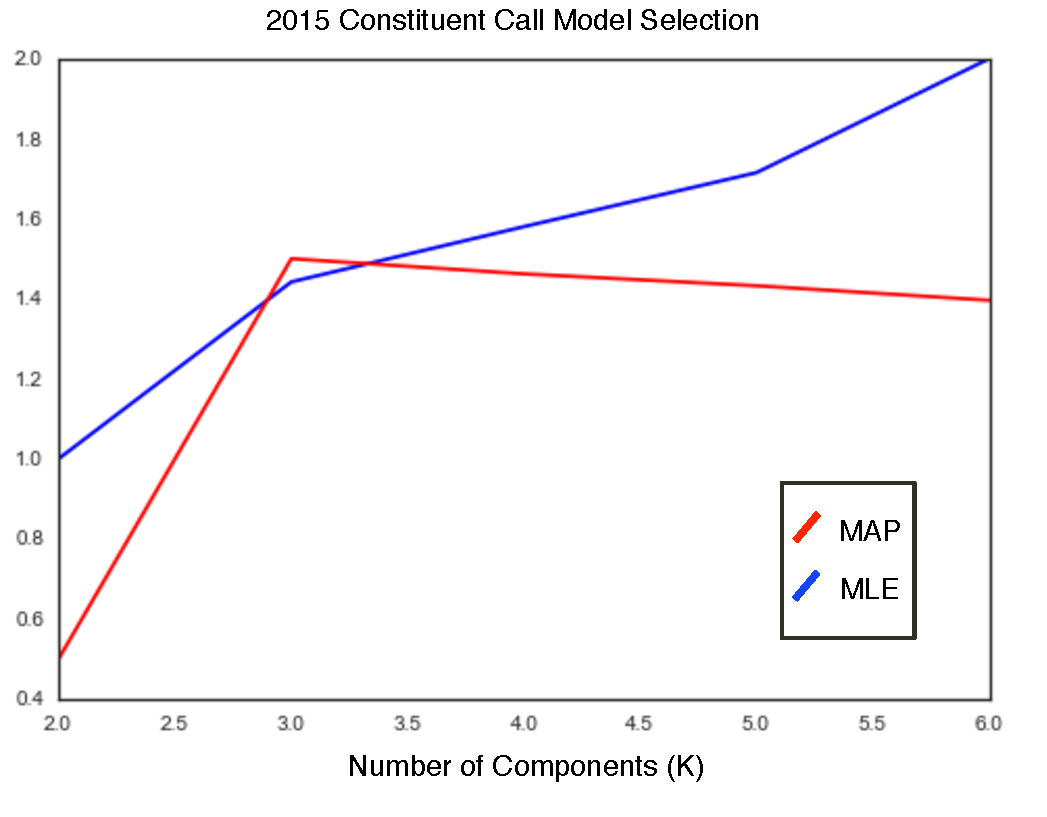
\includegraphics[height=50mm]{Call_bic}}%height=30mm
\hskip1cm
\subfigure[BIC score plot for Citizens Connect Data]{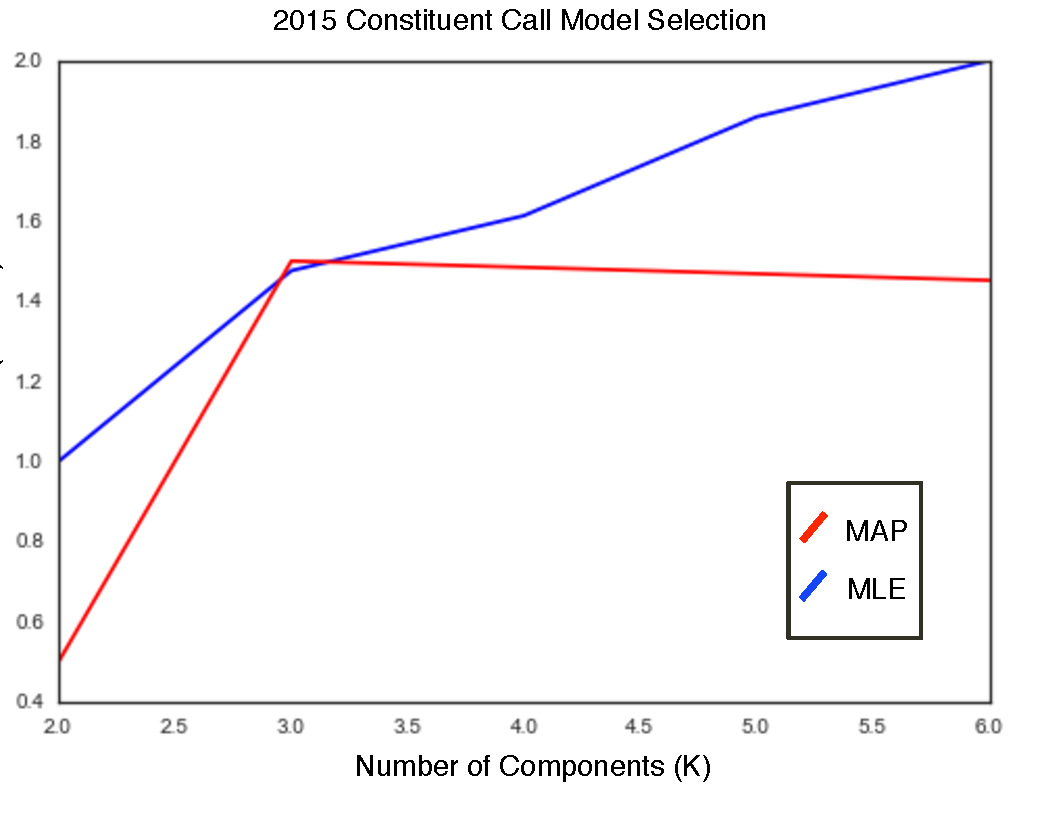
\includegraphics[height=50mm]{App_bic}}%height=30mm
\end{center}\label{fig:bic}
\vskip -0.2in
\end{figure} 


\section{Computing Point Estimates}
We compute point estimates, maximum likelihood and maximum a posteriori estimates, for our model via expectation maximization. We note that EM algorithms are sensitive to initialization. For example, if the means of the components are initialized in such a way where some component is initially assigned few or no points, this will result in the estimates for $\Sigma$ being singular for the next iteration of the algorithm. To address the problem of choosing appropriate initializations, we will use the following initialization regime:
\begin{enumerate}
\item For MLE, we initialize the parameters $\mu$, $\pi$, $\Sigma$ using the means, mixing coefficients and scatter matrices for the components obtained from K-means or simulated annealing. 
\item For MAP, we initialize the hyper-parameters of our model randomly and initialize the parameters $\mu$, $\pi$, $\Sigma$ using MLE estimates.
\end{enumerate}
Observing that MLE tends to overfit for Gaussian mixture models, in the end, we will use the MAP estimate for our cluster analysis (the EM update equations for MLE and MAP are found in the ipython notebook $\texttt{EM for MLE and MAP}$).

Convergence of the algorithms is checked by generating log-likelihood plots (against the number of iterations of the algorithm). The log-likelihood plots for MAP estimates on constituent call and app data is shown in Figure \ref{fig:conv}. The log-likelihood plots for MLE on the data is included in the ipython notebook $\texttt{EM for MLE and MAP}$. 
\begin{figure}[h!]
\begin{center}
\caption{Convergence of EM Algorithms}
\subfigure[Log Likelihood for MAP (Call Data)]{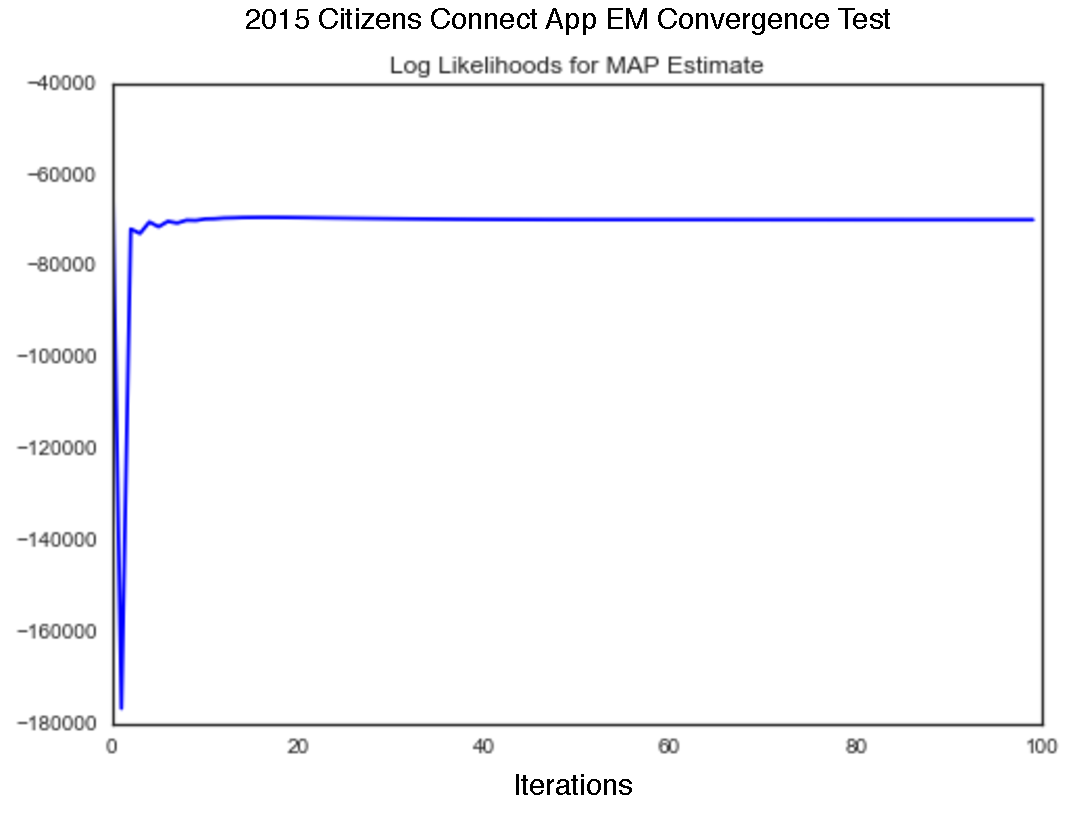
\includegraphics[height=41mm]{call_MAP}}%height=30mm
\hskip1cm
\subfigure[Log Likelihood for MAP (App Data)]{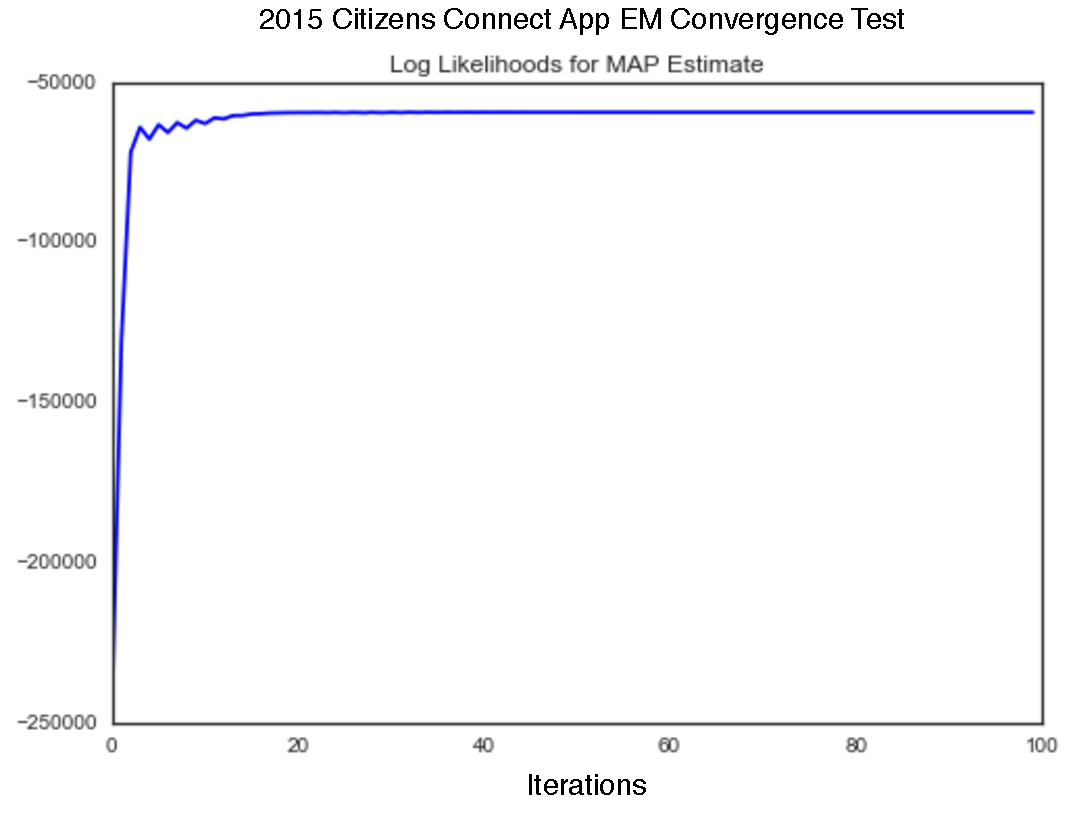
\includegraphics[height=41mm]{app_MAP}}
\end{center}\label{fig:conv}
\vskip -0.2in
\end{figure} 

\section{Cluster Analysis}
Based on our MAP estimate of the model parameters, we produce a hard clustering of our data - each data point, $\mathbf{x}_n$, is attributed to the cluster, $k$ for which $\pi_k p(\mathbf{x}_n | \mu, \Sigma)$ is the largest, over $1\leq k\leq K$. The clustering is visualized on axes: 
\begin{align}
x &= \text{response time (standardized)},\quad y = \text{longitude (standardized)}, \quad z = \text{latitude (standardized)}.
\end{align}

\begin{figure}[h!]
\begin{center}
\caption{Clustering from Point Estimates}
\subfigure[MAP Clustering (Call Data)]{\includegraphics[height=41mm]{3d_call}}%height=30mm
\hskip1cm
\subfigure[MAP Clustering (App Data)]{\includegraphics[height=41mm]{3d_app}}
\end{center}\label{fig:conv}
\vskip -0.2in
\end{figure} 

\begin{figure}[h!]
\begin{center}
\caption{Clustering from Point Estimates}
\subfigure[MAP Clustering (Call Data)]{\includegraphics[height=41mm]{2d_call}}%height=30mm
\hskip1cm
\subfigure[MAP Clustering (App Data)]{\includegraphics[height=41mm]{2d_app}}
\end{center}\label{fig:conv}
\vskip -0.2in
\end{figure} 

\begin{figure}[h!]
\begin{center}
\caption{Clustering from Point Estimates}
\subfigure[MAP Clustering (Call Data)]{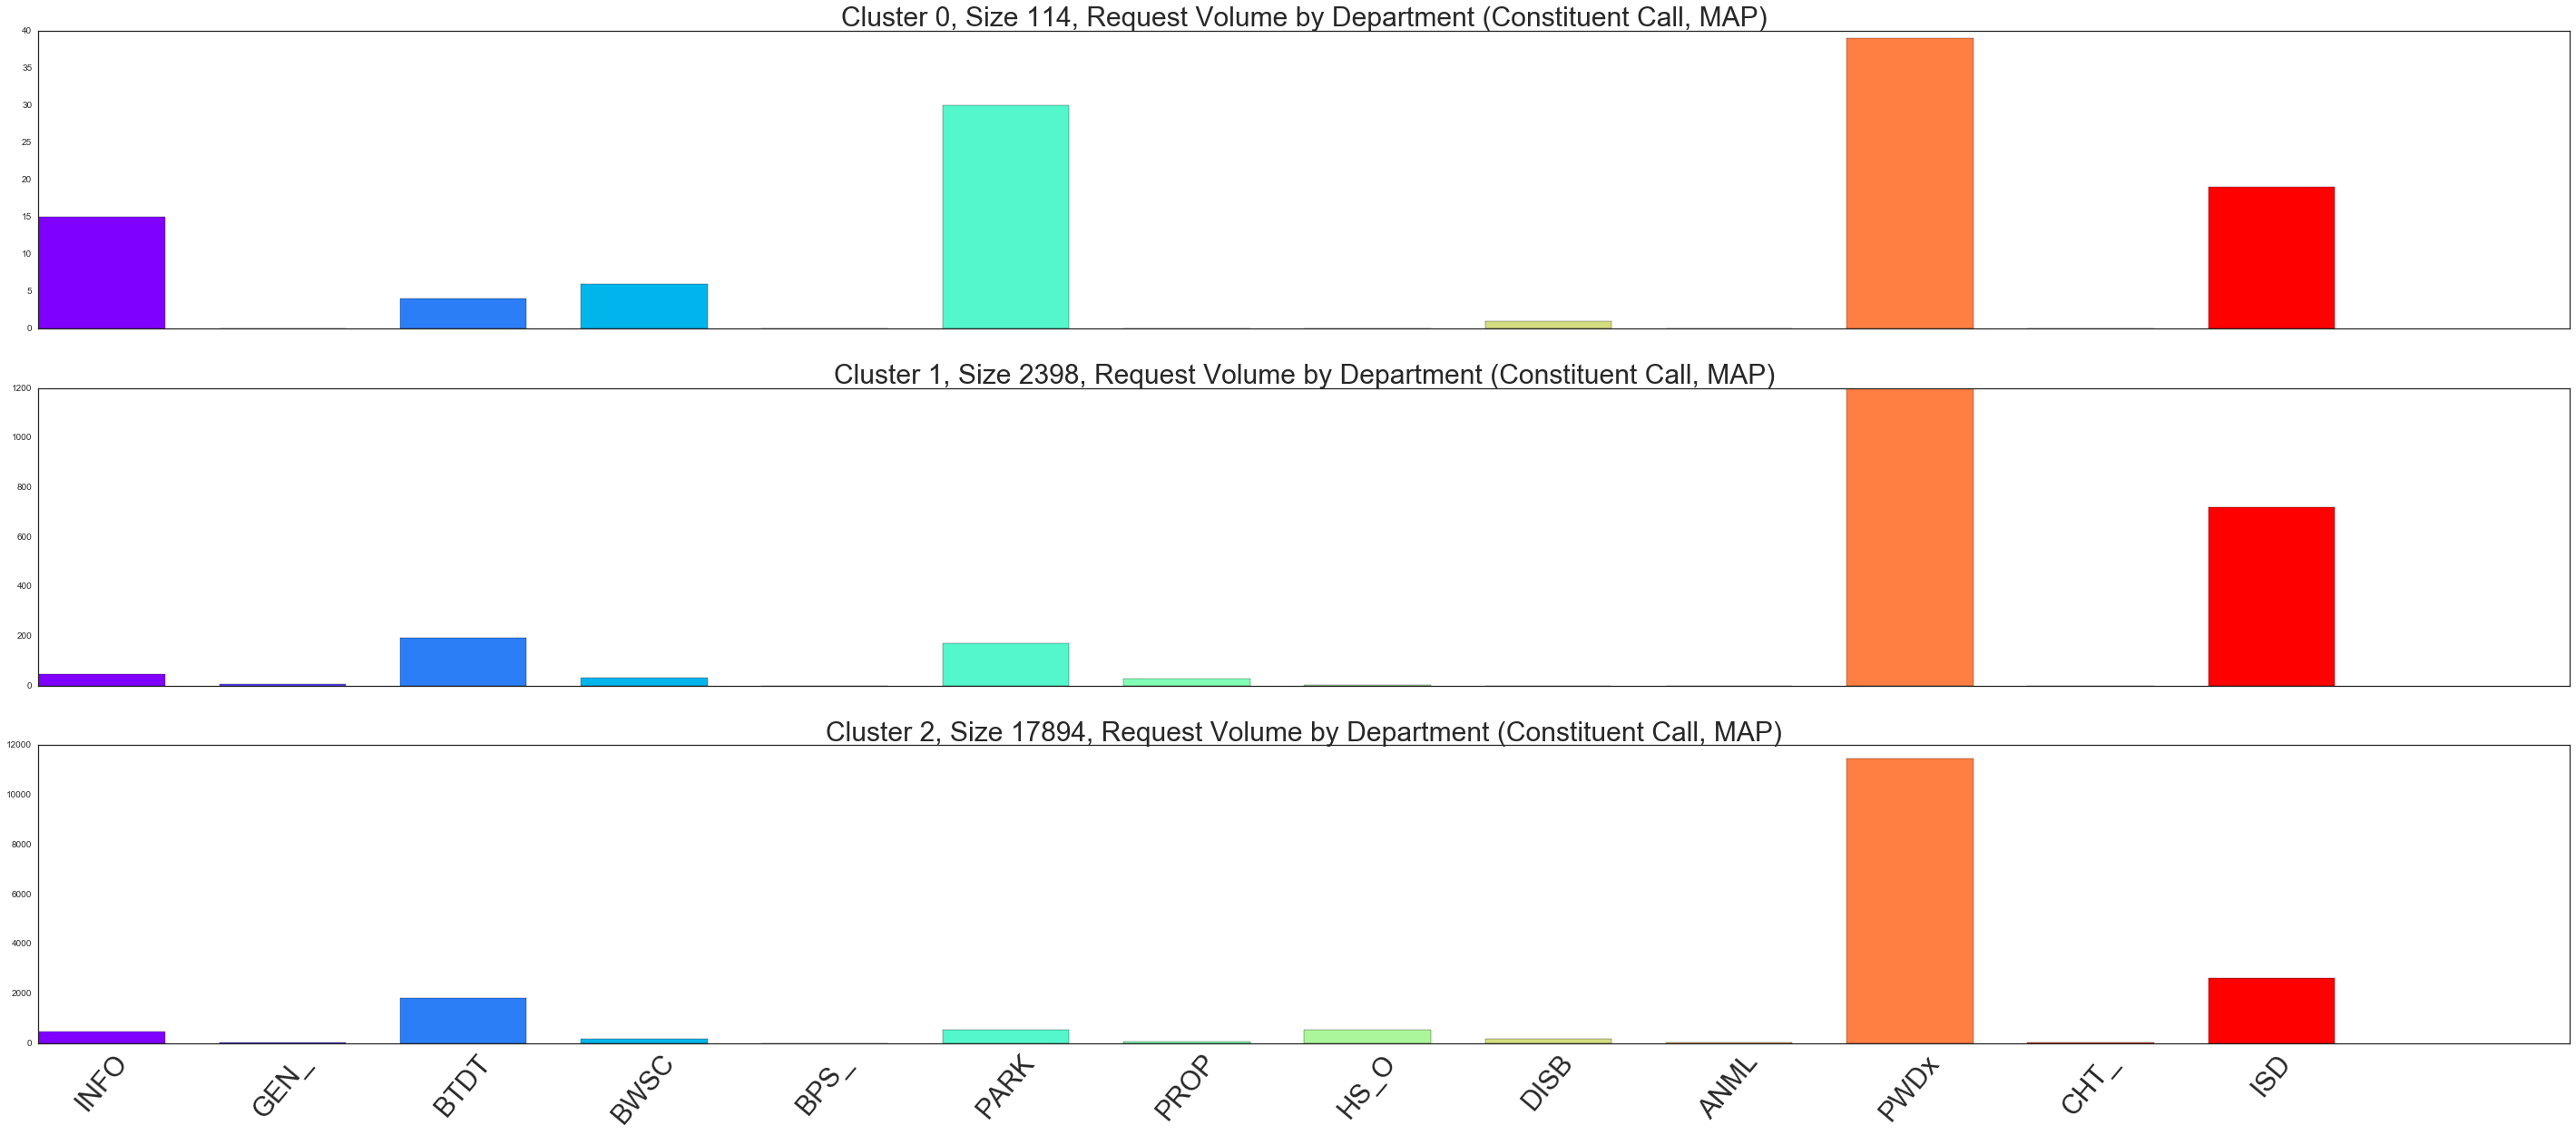
\includegraphics[height=41mm]{profile_call}}%height=30mm
\hskip1cm
\subfigure[MAP Clustering (App Data)]{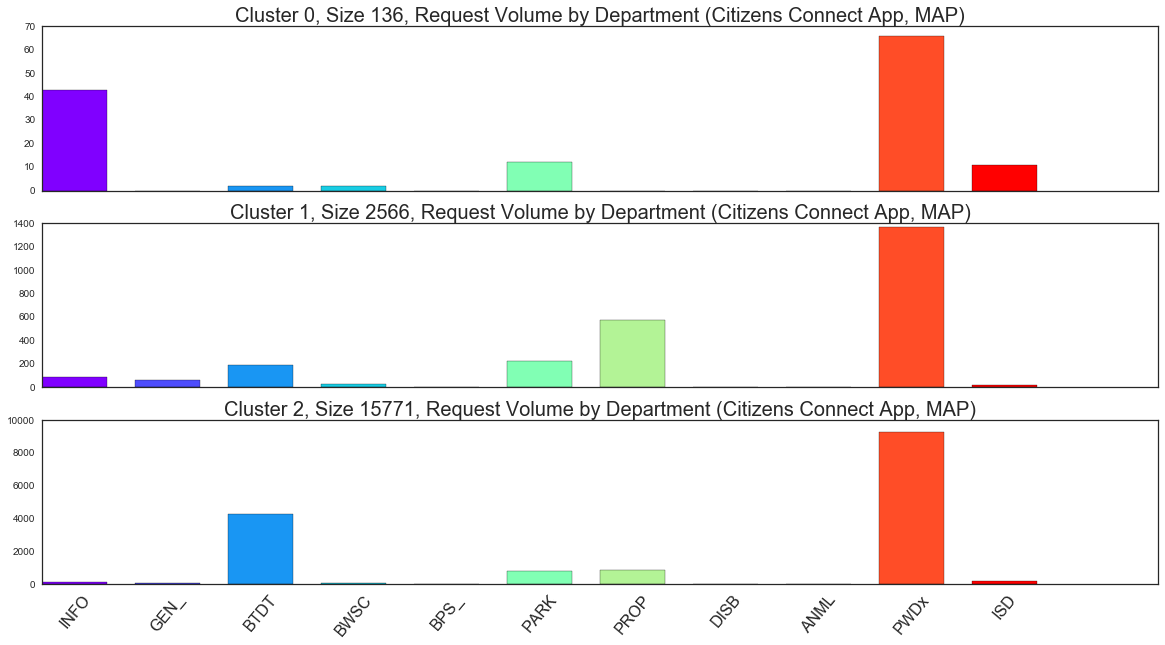
\includegraphics[height=41mm]{profile_app}}
\end{center}\label{fig:conv}
\vskip -0.2in
\end{figure} 

\bibliographystyle{plain}
\bibliography{GMMbib.bib}


\end{document}